\chapter{Agentic AI for Workflow Automation}
\label{ch:agentic}

\section{Introduction and Motivation}
\label{sec:agentic_intro}

Agentic AI extends LLM capabilities beyond single-turn interactions to autonomous, goal-directed behavior. Unlike traditional AI systems with narrowly defined tasks and explicit instructions, agentic AI dynamically reconfigures its strategies based on feedback, uncertainty, and evolving objectives. This makes it particularly valuable for automating complex business workflows that traditionally require human judgment and coordination.

This chapter addresses the second research question (RQ2): \textit{How can multi-agent LLM systems be designed and evaluated for reliable, scalable enterprise automation?} The research presented here builds upon the evaluation methodology established in Chapter~\ref{ch:rag}---particularly the philosophy of multi-dimensional evaluation that integrates quality considerations beyond accuracy---and extends it to the unique challenges of multi-agent coordination. The findings inform deployment strategies examined in Chapter~\ref{ch:strategies}, where reasoning configuration and hardware selection interact to determine system effectiveness.

This chapter presents the design and evaluation of autonomous, LLM-driven multi-agent systems for enterprise workflow automation, synthesizing findings from six peer-reviewed publications:

\begin{enumerate}[leftmargin=*]
    \item \textbf{Invoice Reconciliation System}~\cite{huang2025invoice}: Edge-deployed LLMs in multi-agent systems for SME automation (ICDSAAI 2025)
    \item \textbf{Tool Invocation Reliability Framework}~\cite{huang2026when}: Diagnostic framework for multi-agent systems introducing the 12-category error taxonomy, validated on invoice reconciliation (ICAIBD 2026, submitted)
    \item \textbf{LLM-as-Judge Framework}~\cite{huang2026judge}: Scalable test coverage evaluation with novel Evaluation Completion Rate (ECR@1) metric for operational reliability (AAAI 2026 Workshops, accepted)
    \item \textbf{Automated Acceptance Test Generation}~\cite{huang2026open}: Cooperative multi-agent system for Gherkin test generation using AutoGen Swarm, evaluated using the LLM-as-Judge framework (PAKDD 2026 Workshops, submitted)
    \item \textbf{Hierarchical Multi-Agent System for Payments}~\cite{huang2026hmasp}: End-to-end agentic payment processing with modular architecture (PAKDD 2026, submitted)
    \item \textbf{EdgeAgent Annotation Pipeline}~\cite{huang2026edgeagent}: Semi-automatic data labeling with edge-deployed LLMs, introducing the Agentic Success Rate (ASR) metric for fine-grained reliability evaluation (PAKDD 2026, submitted)
\end{enumerate}

The chapter is organized to highlight methodological progressions: Sections~\ref{sec:invoice_reconciliation}--\ref{sec:diagnostic_framework} present invoice reconciliation and its evolution into a comprehensive diagnostic framework with the 12-category error taxonomy; Sections~\ref{sec:llm_judge}--\ref{sec:cmas4g2} demonstrate how LLM-as-Judge enables automated acceptance test generation; and Sections~\ref{sec:hmasp}--\ref{sec:edgeagent} extend these methodologies to payments and annotation domains.

A key contribution of this chapter is the introduction of two novel metrics that complement the Repetition-Aware Performance (RAP) metric from Chapter~\ref{ch:rag}: the \textbf{Agentic Success Rate (ASR)}, introduced in Section~\ref{sec:edgeagent}, which provides fine-grained evaluation of tool-calling precision in multi-step workflows, and the \textbf{Evaluation Completion Rate (ECR@1)}, which measures first-attempt success rates in automated evaluation systems---both addressing critical gaps in agentic AI evaluation methodology. Together with the 12-category error taxonomy, these metrics enable systematic diagnosis of failure modes impossible with traditional binary success/failure evaluation.

\section{Foundations of Agentic AI}
\label{sec:agentic_foundations}

\subsection{Distinguishing Characteristics}

Agentic AI systems are characterized by several key capabilities that distinguish them from traditional AI applications:

\begin{itemize}[leftmargin=*]
    \item \textbf{Tool Use:} Ability to interact with external tools, APIs, databases, and services
    \item \textbf{Planning:} Decomposing complex goals into executable sub-tasks
    \item \textbf{Memory:} Maintaining state across interactions for long-term objectives
    \item \textbf{Reflection:} Self-evaluation and strategy adjustment based on outcomes
    \item \textbf{Collaboration:} Coordinating with other agents and human operators
\end{itemize}

These capabilities introduce complexity beyond single-turn generation tasks. While Chapter~\ref{ch:rag} addressed optimization challenges for RAG systems involving retrieval and generation, agentic systems must orchestrate multiple tools across multiple steps, with errors in early stages cascading through subsequent operations.

\subsection{Challenges in Enterprise Deployment}

Implementing multi-agent AI systems in enterprise settings presents several challenges~\cite{chawla2024agentic}:

\begin{enumerate}[leftmargin=*]
    \item \textbf{Coordination Complexity:} Managing multiple LLM-powered agents is computationally intensive, raising concerns about latency and resource utilization
    
    \item \textbf{Cost Management:} Costs escalate significantly when relying on proprietary cloud-based LLMs or high-performance infrastructure
    
    \item \textbf{Data Privacy:} Enterprise requirements often necessitate edge deployment, introducing technical complexities
    
    \item \textbf{Reliability:} Agent failures may stem from poor system design rather than model limitations---recent research demonstrates that LLM-based multi-agent system failures often originate from architectural decisions rather than model quality
    
    \item \textbf{Framework Maturity:} Lack of mature orchestration frameworks complicates inter-agent communication
\end{enumerate}

These challenges motivate the systematic evaluation methodology developed in this chapter, where we distinguish between orchestration failures (addressable through better prompting and architecture) and fundamental model limitations (requiring larger models or different approaches).

%% =============================================================================
%% PART 1: Invoice Reconciliation → Diagnostic Framework (Papers 1-2)
%% =============================================================================

\section{Multi-Agent Architecture for Invoice Reconciliation}
\label{sec:invoice_reconciliation}

This section presents the first of two related studies on invoice reconciliation. The initial system~\cite{huang2025invoice} establishes the multi-agent architecture and demonstrates feasibility, while Section~\ref{sec:diagnostic_framework} extends this work with a comprehensive diagnostic framework~\cite{huang2026when} introducing the 12-category error taxonomy for systematic failure characterization.

\subsection{Problem Context}

Invoice reconciliation is a critical yet labor-intensive process for businesses, particularly small and medium-sized enterprises (SMEs). The process involves matching incoming payments to outstanding invoices, cross-verifying databases, emails, and transaction documents, updating associated records and status fields, and handling exceptions and discrepancies.

Traditional automation approaches frequently fall short in handling unstructured data and accommodating complex business rules. Our multi-agent system addresses these challenges through specialized, coordinated LLM agents deployed on edge devices, ensuring data privacy while maintaining high accuracy.

\subsection{System Architecture}

Figure~\ref{fig:invoice_architecture} presents the overall architecture. The system comprises three specialized agents operating sequentially:

\begin{figure}[htbp]
    \centering
    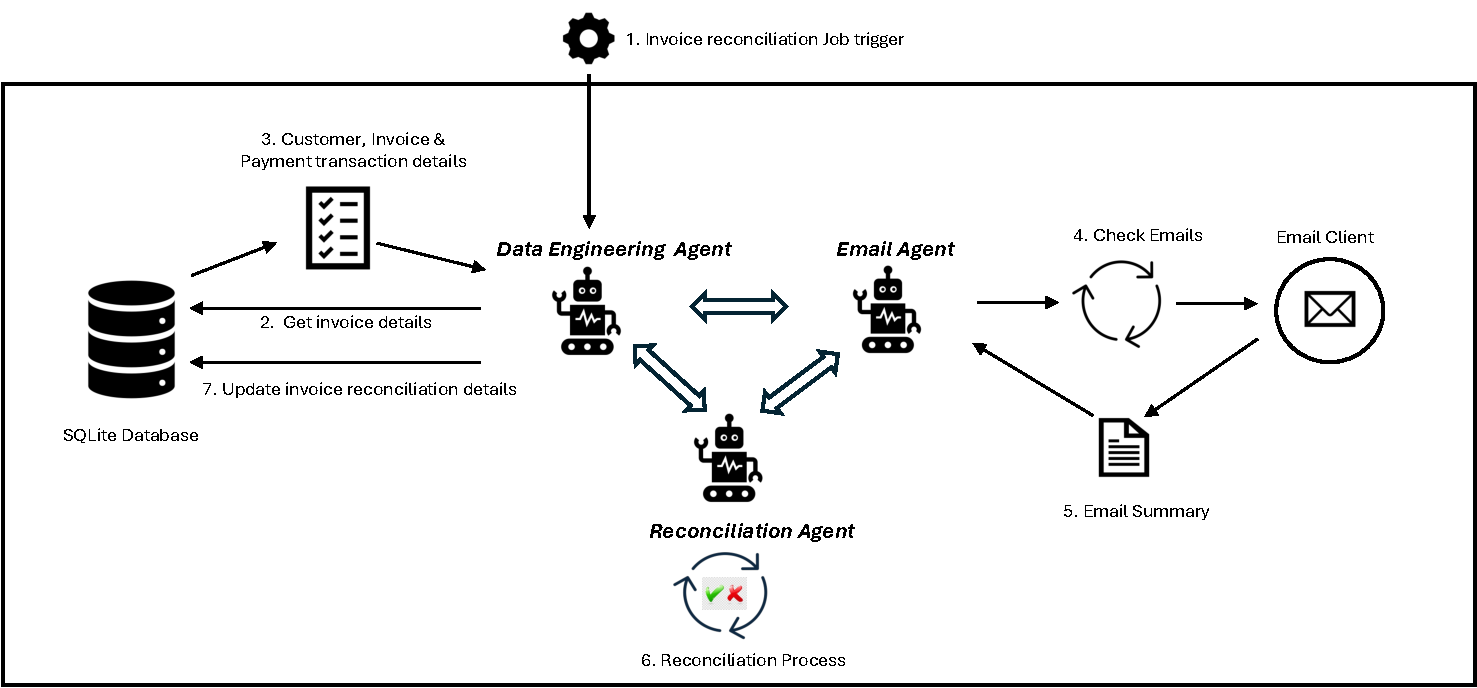
\includegraphics[width=1\textwidth]{images/invoice-rec.pdf}
    \caption{End-to-end workflow of the multi-agent architecture-based invoice reconciliation system.}
    \label{fig:invoice_architecture}
\end{figure}

\subsubsection{Data Engineering Agent}

The Data Engineering Agent serves as an intelligent interface between natural language requests and database operations, utilizing SQLite as an in-memory database for efficient business invoicing data management. Key capabilities include:

\begin{itemize}[leftmargin=*]
    \item Translating natural language queries into SQL commands
    \item Performing schema validation and query verification
    \item Executing queries against SQLite databases
    \item Converting results back to natural language summaries
\end{itemize}

The agent's architecture incorporates two primary tools: an SQL query builder and an SQL query executor, both enhanced by few-shot prompting techniques. These prompts provide essential schema information and example queries, significantly improving the accuracy and reliability of database interactions.

\subsubsection{Email Agent}

The Email Agent processes client communications and attachments through a systematic workflow:

\begin{enumerate}[leftmargin=*]
    \item Establishes live connection with email client via API
    \item Scans inbox for recent emails from customers with ``Unpaid'' status
    \item Checks for attachments and processes them using vision-based OCR
    \item Generates structured summaries of email content and extracted invoice details
\end{enumerate}

Unlike proprietary models that integrate vision capabilities, open-source models such as Functionary V3.1 and Qwen2.5 excel in function calling but lack native vision capabilities. To address this limitation, we supplemented these models with Llama3.2-Vision-11B for robust image processing functionality.

\subsubsection{Reconciliation Agent}

The Reconciliation Agent integrates outputs from other agents and performs the core matching logic:

\begin{itemize}[leftmargin=*]
    \item Combines structured data from Data Engineering and Email Agents
    \item Applies business rules for payment-invoice matching
    \item Updates database records with reconciliation results
    \item Generates status reports and exception notifications
\end{itemize}

\subsection{LangGraph-Based Orchestration}

The system is implemented using the LangGraph framework~\cite{langchain2024langgraph}, which provides graph-based architecture enabling flexible workflows, dynamic execution paths based on intermediate results, modular agent definitions for maintainability, and state management for multi-step processes.

\subsection{Experimental Setup}

\subsubsection{Hardware Configurations}

Testing was conducted on two hardware systems representing typical SME environments:

\begin{enumerate}[leftmargin=*]
    \item \textbf{RTX A6000 Desktop:} Ubuntu via WSL, 48GB VRAM, approximately \$10,000 USD
    \item \textbf{RTX 4090 Laptop:} Ubuntu via WSL, 16GB VRAM, approximately \$5,000 USD
\end{enumerate}

Due to memory constraints, only smaller models (qwen2.5:7b, functionary-small, llama3.2-vision:11b) were evaluated on the RTX 4090, while all open-source models were tested on the RTX A6000. This hardware diversity informs the comprehensive deployment evaluation in Chapter~\ref{ch:strategies}, where we extend benchmarking across six platforms.

\subsubsection{Model Selection}

Table~\ref{tab:agentic_models} lists evaluated models.

\begin{table}[htbp]
\centering
\caption{Models Evaluated for Multi-Agent Invoice Reconciliation}
\label{tab:agentic_models}
\begin{tabular}{@{}llcc@{}}
\toprule
\textbf{Model} & \textbf{Type} & \textbf{Parameters} & \textbf{Hardware} \\
\midrule
GPT-4o & Proprietary (API) & Unknown & Cloud \\
GPT-4o-mini & Proprietary (API) & Unknown & Cloud \\
Qwen2.5-72B & Open-source & 72B & RTX A6000 \\
Qwen2.5-32B & Open-source & 32B & RTX A6000 \\
Qwen2.5-7B & Open-source & 7B & Both \\
Functionary-medium & Open-source & 70B & RTX A6000 \\
Functionary-small & Open-source & 8B & Both \\
Llama3.2-vision:11B & Open-source & 11B & RTX A6000 \\
\bottomrule
\end{tabular}
\end{table}

\subsubsection{Evaluation Metrics}

\begin{itemize}[leftmargin=*]
    \item \textbf{Success Rate:} Proportion of correctly completed reconciliation tasks
    \item \textbf{Mean Execution Time:} Average time per reconciliation workflow
    \item \textbf{Energy per Task:} Joules consumed per completed task
    \item \textbf{Performance-to-Power Ratio:} Success rate normalized by energy consumption
\end{itemize}

\subsection{Results}

Table~\ref{tab:invoice_results} presents comprehensive evaluation results.

\begin{table}[htbp]
\centering
\caption{Invoice Reconciliation Performance Across Models and Platforms}
\label{tab:invoice_results}
\begin{tabular}{@{}llccc@{}}
\toprule
\textbf{Model} & \textbf{Platform} & \textbf{SUCCESS} & \textbf{NO INVOICE} & \textbf{ERROR} \\
\midrule
GPT-4o (API) & Cloud & 93.13\% & -- & -- \\
GPT-4o-mini (API) & Cloud & 97.68\% & -- & -- \\
qwen2.5:7b & RTX 4090 & 865 & 2 & 123 \\
qwen2.5:7b & RTX A6000 & 850 & 4 & 136 \\
functionary-small & RTX 4090 & 879 & 101 & 10 \\
functionary-small & RTX A6000 & 876 & 108 & 6 \\
qwen2.5:32b & RTX A6000 & \textbf{989} & 0 & 1 \\
functionary-medium & RTX A6000 & 932 & 47 & 11 \\
qwen2.5:72b & RTX A6000 & 985 & 1 & 4 \\
\bottomrule
\end{tabular}
\end{table}

Key findings:

\begin{enumerate}[leftmargin=*]
    \item \textbf{Open-source superiority:} Qwen2.5-32B achieved 99.9\% success rate (989/990), outperforming all proprietary alternatives including GPT-4o-mini (97.68\%). This finding parallels the Orca-2 results from Chapter~\ref{ch:rag}, where smaller open-source models outperformed GPT-4 on RAG tasks, reinforcing the theme that architecture and training methodology matter more than parameter count or proprietary status.
    
    \item \textbf{Execution time parity:} Edge-deployed Qwen2.5-32B execution times were comparable to cloud APIs, making it a superior candidate due to combined accuracy and speed advantages
    
    \item \textbf{Resource efficiency:} Functionary-small achieved optimal performance-to-power ratio, consuming only 523J per task on RTX 4090 while maintaining 88.78\% success rate
    
    \item \textbf{Energy trade-offs:} Larger models consume substantially more energy (19,394J for qwen2.5:72b vs 523J for functionary-small) with diminishing accuracy returns
    
    \item \textbf{Platform variations:} RTX 4090 achieved higher success rates for qwen2.5:7b and functionary-small compared to RTX A6000, underscoring its suitability for edge applications
\end{enumerate}

\subsection{Error Analysis}

Workflow outputs were categorized into three groups:

\textbf{SUCCESS:} Correctly located, identified, and processed invoice data. The workflow performed as expected, handling data extraction and reconciliation seamlessly.

\textbf{NO INVOICE:} Workflow failures due to OCR task failures (LLM hallucinations extracting non-existent information from images) or reconciliation task failures (LLM misinterpreting natural language queries and generating invalid SQL queries).

\textbf{ERROR:} Complete task failures from fundamental context misunderstanding, where the LLM completely misinterpreted workflow requirements.

Error trends across model families revealed that functionary models recorded higher NO INVOICE cases, indicating potential limitations in handling certain data reconciliation scenarios. Conversely, qwen2.5 family models exhibited greater ERROR occurrences, suggesting challenges in interpreting task context accurately.

While this initial study demonstrated the feasibility of edge-deployed multi-agent systems for invoice reconciliation, the coarse-grained error categories (SUCCESS, NO INVOICE, ERROR) limited our ability to diagnose specific failure modes. This motivated the development of the comprehensive diagnostic framework presented in the following section.

%% =============================================================================
%% Section: Diagnostic Framework - Building on Invoice Reconciliation
%% =============================================================================

\section{When Agents Fail to Act: Diagnostic Framework for Tool Invocation Reliability}
\label{sec:diagnostic_framework}

Building upon the invoice reconciliation system presented in Section~\ref{sec:invoice_reconciliation}, this section introduces a comprehensive diagnostic framework~\cite{huang2026when} that addresses a critical limitation of the initial study: the inability to systematically diagnose \textit{where} and \textit{why} workflows fail. Traditional binary success/failure metrics obscure critical diagnostic information, limiting opportunities for targeted improvements.

This diagnostic approach parallels the philosophy underlying the RAP metric from Chapter~\ref{ch:rag}: just as RAP integrates repetition quality into performance evaluation to enable principled hyperparameter tuning, our error taxonomy integrates failure mode characterization into system evaluation to enable principled architecture decisions.

\subsection{Motivation and Gap Analysis}

Current evaluation approaches for multi-agent LLM systems predominantly report aggregate task success rates~\cite{hendrycks2021measuring,zheng2024judging}, obscuring underlying failure causes. While recent work by Kokane et al.~\cite{kokane2024spectool} demonstrates the value of granular error taxonomies for single-agent tool use, these frameworks remain insufficient for multi-agent contexts where failures cascade through coordination protocols.

Consider the invoice reconciliation pipeline from Section~\ref{sec:invoice_reconciliation}: a model might correctly invoke the OCR tool but fail to initiate the subsequent database update, resulting in pipeline failure. Binary metrics would score this as complete failure, obscuring that the model successfully executed partial workflow steps---a fundamentally different (and more easily addressable) problem than complete workflow incomprehension.

This diagnostic gap has significant practical implications:
\begin{itemize}[leftmargin=*]
    \item \textbf{Model selection:} Organizations cannot determine whether failures stem from model capacity limitations or prompt design issues
    \item \textbf{System improvement:} Without granular failure characterization, developers cannot prioritize optimization efforts
    \item \textbf{Deployment decisions:} Binary metrics provide insufficient information for evidence-based deployment planning across hardware configurations
\end{itemize}

\subsection{Diagnostic Framework Overview}

Our diagnostic framework provides systematic methodology for evaluating procedural reliability in multi-agent LLM systems through two core components:

\begin{enumerate}[leftmargin=*]
    \item \textbf{12-Category Error Taxonomy:} Comprehensive failure characterization spanning tool initialization, parameter handling, execution, and result interpretation
    \item \textbf{Hardware-Performance Characterization:} Systematic evaluation across deployment configurations for deployment guidance
\end{enumerate}

The framework is designed for broad applicability across multi-agent scenarios while maintaining diagnostic precision through domain-specific instantiation. We validate this approach using the invoice reconciliation system from Section~\ref{sec:invoice_reconciliation}, demonstrating how the framework transforms coarse error categories into actionable diagnostics.

\subsection{12-Category Error Taxonomy}

For comprehensive failure characterization in multi-agent coordination scenarios, we develop a systematic error taxonomy. The taxonomy combines four error types with three tool categories, yielding twelve distinct failure modes.

\paragraph{Error Type Categories.}

\begin{itemize}[leftmargin=*]
    \item \textbf{Not Initialized:} Agent fails to properly invoke tool due to malformed calls, incorrect tool names, or invalid parameter structures
    \item \textbf{Args Mismatch:} Tool invocation succeeds but contains incorrect or invalid arguments leading to tool-specific failures
    \item \textbf{Error:} Tool executes with valid parameters but returns runtime errors or exceptions
    \item \textbf{Result Mismatch:} Tool execution succeeds but produces outputs that cause downstream task failure
\end{itemize}

\paragraph{Tool Categories.} For invoice reconciliation workflows, we define three tool categories representing common primitives in structured business automation:
\begin{itemize}[leftmargin=*]
    \item \textbf{OCR Tool:} Multi-modal document processing for receipt and invoice image analysis
    \item \textbf{DB Query Tool:} Database query operations for invoice lookup and verification
    \item \textbf{DB Update Tool:} Database modification operations for status updates
\end{itemize}

\paragraph{Complete Taxonomy.} The cross-product produces twelve diagnostic categories:

\begin{enumerate}[leftmargin=*]
    \item \texttt{OCR\_TOOL\_NOT\_INITIALIZED}: Failure to invoke OCR tool
    \item \texttt{OCR\_TOOL\_ARGS\_MISMATCH}: OCR tool called with invalid arguments
    \item \texttt{OCR\_TOOL\_ERROR}: OCR tool execution returns runtime errors
    \item \texttt{OCR\_TOOL\_RESULT\_MISMATCH}: OCR output causes downstream failures
    \item \texttt{DB\_QUERY\_TOOL\_NOT\_INITIALIZED}: Failure to invoke database query tool
    \item \texttt{DB\_QUERY\_TOOL\_ARGS\_MISMATCH}: Query tool called with invalid arguments
    \item \texttt{DB\_QUERY\_TOOL\_ERROR}: Query execution returns runtime errors
    \item \texttt{DB\_QUERY\_TOOL\_RESULT\_MISMATCH}: Query results cause downstream failures
    \item \texttt{DB\_UPDATE\_TOOL\_NOT\_INITIALIZED}: Failure to invoke database update tool
    \item \texttt{DB\_UPDATE\_TOOL\_ARGS\_MISMATCH}: Update tool called with invalid arguments
    \item \texttt{DB\_UPDATE\_TOOL\_ERROR}: Update execution returns runtime errors
    \item \texttt{DB\_UPDATE\_TOOL\_RESULT\_MISMATCH}: Update results cause downstream failures
\end{enumerate}

This taxonomy enables systematic identification of reliability bottlenecks and provides actionable diagnostic information for system improvement beyond aggregate success metrics.

\subsection{Experimental Methodology}

\subsubsection{Enhanced Multi-Agent Architecture}

We validate the diagnostic framework using the invoice reconciliation architecture from Section~\ref{sec:invoice_reconciliation}, enhanced with detailed instrumentation for failure diagnosis. Each agent is augmented with logging mechanisms to capture initialization failures, parameter mismatches, and execution errors at each tool invocation.

\subsubsection{Expanded Model Selection}

To establish comprehensive reliability benchmarks across the performance spectrum, we expand evaluation to include:

\begin{itemize}[leftmargin=*]
    \item \textbf{Closed-Source Models:} OpenAI's GPT-4 series (gpt-4o, gpt-4o-mini, gpt-4.1-nano, gpt-4.1-mini, gpt-4.1) and Anthropic's Claude models (3.5 Sonnet, 3.7 Sonnet) serve as reference baselines representing state-of-the-art proprietary systems
    \item \textbf{Open-Weight Models:} The Qwen2.5 series (3B, 7B, 14B, 32B, 72B) and Functionary V3.1 (8B, 70B) provide systematic coverage across model scales, with local deployment ensuring data sovereignty
\end{itemize}

All open-weight models were executed locally using Ollama v0.6.8 with 4-bit quantization (Q4\_K\_M format) to simulate realistic edge deployment constraints.

\subsubsection{Extended Hardware Infrastructure}

We extend testing to three representative edge platforms:

\begin{itemize}[leftmargin=*]
    \item \textbf{NVIDIA RTX A6000 Ada GPU:} High-end workstation (48GB VRAM, Ubuntu 24.04, \textasciitilde\$10K)
    \item \textbf{NVIDIA GeForce RTX 4090 Laptop GPU:} Mobile workstation (16GB VRAM, Ubuntu 24.04 via WSL, \textasciitilde\$5K)
    \item \textbf{Apple M3 Max:} Consumer-grade ARM platform (96GB unified memory, macOS 15.4.1, \textasciitilde\$4K)
\end{itemize}

\subsubsection{Evaluation Dataset and Protocol}

We employ standardized evaluation using a synthetic dataset of 1,980 test instances balanced between vision-enabled (990) and text-only (990) tasks. All experiments employ deterministic execution (temperature=0, fixed prompts), eliminating sampling variance and ensuring reproducible diagnostic assessment.

\subsection{Results and Analysis}

\subsubsection{Performance and Reliability Trade-offs}

Table~\ref{tab:asr_overall_performance} summarizes overall performance metrics across all evaluated LLM configurations.

\begin{table}[htbp]
\centering
\caption{Overall Invoice Reconciliation Performance Across LLM Configurations. SR = Success Rate. All metrics based on 1,980 test instances.}
\label{tab:asr_overall_performance}
\begin{tabular}{@{}llccc@{}}
\toprule
\textbf{Model} & \textbf{Platform} & \textbf{SR (\%)} & \textbf{Time (s)} & \textbf{Steps} \\
\midrule
\multicolumn{5}{l}{\textit{Closed-source models}} \\
gpt-4o-mini & OpenAI & 99.3 & 7.6 $\pm$ 1.6 & 8.6 $\pm$ 1.2 \\
gpt-4o & OpenAI & 98.8 & 12.4 $\pm$ 13.2 & 8.5 $\pm$ 0.6 \\
gpt-4.1-nano & OpenAI & 85.7 & 8.6 $\pm$ 12.3 & 18.5 $\pm$ 18.6 \\
gpt-4.1-mini & OpenAI & 99.5 & 8.6 $\pm$ 2.7 & 9.6 $\pm$ 1.9 \\
gpt-4.1 & OpenAI & \textbf{100.0} & 8.3 $\pm$ 7.7 & 9.9 $\pm$ 9.7 \\
claude-3-5-sonnet & Anthropic & 97.8 & 18.7 $\pm$ 6.3 & 8.5 $\pm$ 0.5 \\
claude-3-7-sonnet & Anthropic & 99.3 & 16.8 $\pm$ 12.3 & 8.5 $\pm$ 0.7 \\
\midrule
\multicolumn{5}{l}{\textit{Open-weight models}} \\
qwen2.5:3b & RTX A6000 & 13.9 & 8.1 $\pm$ 19.0 & 18.8 $\pm$ 14.7 \\
qwen2.5:7b & RTX A6000 & 57.3 & 9.9 $\pm$ 10.2 & 20.7 $\pm$ 22.0 \\
qwen2.5:14b & RTX A6000 & 96.6 & \textbf{7.3 $\pm$ 8.0} & 8.6 $\pm$ 2.2 \\
qwen2.5:32b & RTX A6000 & \textbf{100.0} & 13.9 $\pm$ 16.9 & 8.5 $\pm$ 0.5 \\
qwen2.5:72b & RTX A6000 & 95.1 & 39.3 $\pm$ 24.8 & 8.7 $\pm$ 4.2 \\
functionary-small & RTX A6000 & 7.5 & 4.0 $\pm$ 21.6 & 5.6 $\pm$ 3.7 \\
functionary-medium & RTX A6000 & 53.2 & 30.8 $\pm$ 242.6 & 7.8 $\pm$ 2.8 \\
\bottomrule
\end{tabular}
\end{table}

\paragraph{Reliability Thresholds.} Our analysis reveals clear performance thresholds informing deployment decisions:

\begin{itemize}[leftmargin=*]
    \item \textbf{Flawless performance:} qwen2.5:32b achieves perfect 100\% success matching GPT-4.1, demonstrating that open-weight models can achieve closed-source reliability at sufficient scale
    \item \textbf{Production threshold:} qwen2.5:14b maintains 96.6--97.4\% success across all hardware platforms, establishing a practical reliability threshold for cost-sensitive deployments
    \item \textbf{Diminishing returns:} qwen2.5:72b exhibits slightly lower success (95.1\%) than its 32B counterpart, echoing the scaling law findings from Chapter~\ref{ch:rag} where larger models do not always outperform smaller alternatives
    \item \textbf{Fundamental limits:} Smaller models exhibit significant degradation---qwen2.5:7b achieves 49.3--58.5\%, while qwen2.5:3b drops to 13.1--14.9\%---highlighting fundamental capacity constraints in complex multi-agent coordination
\end{itemize}

\paragraph{Hardware Impact on Deployment Viability.} Platform selection critically affects both latency and reliability. qwen2.5:14b executes in 7.3 seconds on RTX A6000 versus 60.0 seconds on M3 Max---an 8.2$\times$ difference highlighting the importance of optimized hardware. However, hardware alone is insufficient: qwen2.5:7b on M3 Max averages 85.9 seconds despite smaller size, requiring 20.7 steps per task versus 8.6 steps for the larger 14B model. Execution logs show that qwen2.5:7b often enters cyclical decision loops, occasionally exceeding LangGraph's recursion limit (25 steps) and triggering forced termination---suggesting that planning efficiency improves with model capacity.

\subsubsection{Diagnostic Error Analysis}

Tables~\ref{tab:asr_error_vision} and~\ref{tab:asr_error_nonvision} present detailed error distributions across all evaluated models, categorized according to our 12-category taxonomy.

\begin{table}[htbp]
\centering
\caption{Error Counts and Rates for Vision Tasks (990 instances). NI = NOT\_INITIALIZED, AM = ARGS\_MISMATCH.}
\label{tab:asr_error_vision}
\small
\resizebox{\textwidth}{!}{%
\begin{tabular}{@{}ll|cc|cc|cc@{}}
\toprule
\textbf{Platform} & \textbf{Model} & \textbf{OCR NI} & \textbf{OCR AM} & \textbf{DB-Q NI} & \textbf{DB-Q AM} & \textbf{DB-U NI} & \textbf{DB-U AM} \\
\midrule
\multirow{5}{*}{RTX A6000} 
 & qwen2.5:3b & 0 & 1 & 0 & 7 & 881 (89\%) & 30 \\
 & qwen2.5:7b & 369 (37\%) & 0 & 151 (15\%) & 21 & 30 & 2 \\
 & qwen2.5:14b & 0 & 0 & 38 (4\%) & 0 & 15 (2\%) & 0 \\
 & qwen2.5:32b & 0 & 0 & 0 & 0 & 0 & 0 \\
 & qwen2.5:72b & 0 & 0 & 28 (3\%) & 0 & 12 (1\%) & 0 \\
\midrule
\multirow{3}{*}{OpenAI} 
 & gpt-4.1-nano & 0 & 0 & 0 & 60 (6\%) & 20 (2\%) & 9 \\
 & gpt-4.1-mini & 0 & 0 & 0 & 0 & 9 (1\%) & 0 \\
 & gpt-4.1 & 0 & 0 & 0 & 0 & 0 & 0 \\
\midrule
\multirow{2}{*}{Anthropic} 
 & claude-3-5-sonnet & 0 & 0 & 0 & 1 & 0 & 29 (3\%) \\
 & claude-3-7-sonnet & 1 & 0 & 1 & 0 & 5 & 0 \\
\bottomrule
\end{tabular}
}
\end{table}

\begin{table}[htbp]
\centering
\caption{Error Counts and Rates for Non-Vision Tasks (990 instances). NI = NOT\_INITIALIZED, AM = ARGS\_MISMATCH.}
\label{tab:asr_error_nonvision}
\small
\begin{tabular}{@{}ll|cc|cc@{}}
\toprule
\textbf{Platform} & \textbf{Model} & \textbf{DB-Q NI} & \textbf{DB-Q AM} & \textbf{DB-U NI} & \textbf{DB-U AM} \\
\midrule
\multirow{5}{*}{RTX A6000} 
 & qwen2.5:3b & 7 (1\%) & 17 (2\%) & 756 (76\%) & 5 \\
 & qwen2.5:7b & 264 (27\%) & 0 & 7 (1\%) & 1 \\
 & qwen2.5:14b & 8 (1\%) & 1 & 4 & 1 \\
 & qwen2.5:32b & 0 & 0 & 0 & 0 \\
 & qwen2.5:72b & 57 (6\%) & 0 & 0 & 0 \\
\midrule
\multirow{3}{*}{OpenAI} 
 & gpt-4.1-nano & 55 (6\%) & 24 (2\%) & 114 (12\%) & 1 \\
 & gpt-4.1-mini & 0 & 0 & 0 & 0 \\
 & gpt-4.1 & 0 & 0 & 0 & 0 \\
\midrule
\multirow{2}{*}{Anthropic} 
 & claude-3-5-sonnet & 0 & 0 & 0 & 9 (1\%) \\
 & claude-3-7-sonnet & 0 & 0 & 1 & 0 \\
\bottomrule
\end{tabular}
\end{table}

\textit{Note: ERROR and RESULT\_MISMATCH categories (4 of 12 taxonomy categories) recorded zero occurrences across all configurations, likely reflecting the deterministic nature of local database operations.}

\paragraph{Systematic Failure Patterns.} Tool initialization failures (\texttt{NOT\_INITIALIZED}) dominate error distributions across all model scales. This pattern holds consistently for both vision and non-vision tasks, indicating that procedural invocation---not parameter handling or result interpretation---represents the primary reliability bottleneck. This suggests fundamental challenges in multi-agent orchestration rather than modality-specific limitations.

\paragraph{Model Scale Impact.} Error rates demonstrate clear inverse correlation with model parameters:

\begin{itemize}[leftmargin=*]
    \item \textbf{Catastrophic failure:} qwen2.5:3b exhibits 881 database update initialization errors (89\% of vision tasks)
    \item \textbf{Moderate improvement:} qwen2.5:14b reduces this to 15--38 errors (1.5--3.8\%)
    \item \textbf{Flawless performance:} qwen2.5:32b achieves zero errors across all categories, matching GPT-4.1
\end{itemize}

This dramatic improvement establishes clear capacity thresholds for production deployment.

\paragraph{Framework Validation.} The systematic patterns revealed by our taxonomy demonstrate its diagnostic value. Traditional aggregate success metrics would obscure the critical insight that tool initialization---rather than execution complexity or result interpretation---represents the primary reliability challenge. This granular understanding enables evidence-based decisions about model selection, system architecture, and deployment strategies impossible with coarse-grained evaluation alone.

\subsubsection{Qualitative Failure Analysis}

To complement quantitative taxonomy results, we conducted systematic qualitative analysis of 200 randomly sampled initialization failures from qwen2.5:3b, qwen2.5:7b, and Functionary-Small execution logs.

\paragraph{Failure Mode Classification.} Our qualitative review identifies two dominant failure patterns:

\textbf{Omission Failures ($\approx$68\% of sampled cases).} Agents fail to recognize that tool invocation is required, producing natural-language responses instead. This reflects inadequate procedural reasoning---the model conceptually resolves the task but omits the necessary operational step, revealing weak coupling between semantic understanding and action execution.
    
\textbf{Malformed Call Failures ($\approx$32\% of sampled cases).} Models correctly identify tool-use needs but construct invalid function calls through incorrect tool names, invalid JSON structure, or hallucinated parameters. These patterns indicate insufficient schema grounding and weak syntactic discipline during tool invocation.

\subsection{Deployment Tiers and Practical Guidance}

Results enable clear deployment guidance based on diagnostic analysis:

\paragraph{Tier 1: Maximum Reliability ($\geq$32B parameters).} Models demonstrate production-ready error profiles with zero errors across all taxonomy categories. qwen2.5:32b on RTX A6000 (\textasciitilde\$10K) achieves flawless performance comparable to GPT-4.1 while maintaining data sovereignty. Appropriate for autonomous workflows requiring high reliability.

\paragraph{Tier 2: Balanced Performance (14B parameters).} qwen2.5:14b represents the minimum viable production configuration, achieving 96.6--97.4\% success across all hardware platforms. On RTX 4090 (\textasciitilde\$5K), it provides 96.6\% reliability with 7.3s latency---the optimal choice for most SME deployments balancing cost, performance, and accuracy.

\paragraph{Tier 3: Budget-Constrained ($<$14B parameters).} Models below 14B require substantial architectural augmentation to achieve acceptable reliability, including validation layers, automated retry mechanisms, and human-in-the-loop escalation.

%% =============================================================================
%% PART 2: LLM-as-Judge → Acceptance Test Generation (Papers 3-4)
%% =============================================================================

\section{LLM-as-Judge for Automated Evaluation}
\label{sec:llm_judge}

This section presents the first of two related studies on automated software quality assurance. The LLM-as-Judge framework~\cite{huang2026judge} establishes methodology for scalable test coverage evaluation, introducing the Evaluation Completion Rate (ECR@1) metric for operational reliability. Section~\ref{sec:cmas4g2} then demonstrates how this framework enables practical automated acceptance test generation~\cite{huang2026open}.

\subsection{Motivation}

As agentic systems scale, manual evaluation becomes impractical. Assessing software test coverage at scale remains a bottleneck in QA pipelines. Traditional static analysis tools (JaCoCo~\cite{crap4j2010}, coverage.py~\cite{coveragepy}, and Istanbul~\cite{istanbul}) provide quantitative metrics but cannot assess semantic completeness---whether tests adequately capture business requirements, edge cases, and error conditions. Manual expert evaluation is accurate but prohibitively expensive at scale.

LLMs offer potential for automated semantic evaluation, but systematic investigation of accuracy, cost, and operational reliability for software testing remains limited. Our LLM-as-Judge (LAJ) framework addresses this gap with rubric-driven assessment aligned with industry best practices.

\subsection{Framework Design}

\subsubsection{Design Principles}

The LAJ framework emphasizes three core principles:

\begin{enumerate}[leftmargin=*]
    \item \textbf{Agreement with humans:} Rubric-grounded scoring aligning with expert judgment
    \item \textbf{Structured outputs:} JSON-formatted responses enabling programmatic processing
    \item \textbf{Deployment awareness:} Metrics capturing operational reality beyond accuracy
\end{enumerate}

\subsubsection{Evaluation Task}

Given a software requirement specification $R$ (e.g., a Jira ticket) and corresponding Gherkin acceptance test script $T$, the LAJ model $M$ produces assessment $A_M(R, T) \in [0, 100]$ representing estimated coverage percentage. We evaluate against expert-provided ground truth $A^*(R, T)$.

\subsection{Novel Reliability Metrics}

Beyond traditional accuracy, we introduce metrics capturing operational reliability:

\subsubsection{Evaluation Completion Rate (ECR@1)}

ECR@1 measures the percentage of evaluations producing valid, parseable output on the first attempt:

\begin{equation}
\text{ECR@1} = \frac{\text{Number of successful first attempts}}{N} \times 100\%
\end{equation}

Reliability failures include API timeouts, malformed JSON, and schema violations. ECR@1 reveals operational reliability variations from 85.4\% to 100\% across models---with direct cost implications through retry overhead.

This metric complements the diagnostic framework from Section~\ref{sec:diagnostic_framework}: while the 12-category taxonomy diagnoses \textit{what} fails in multi-agent workflows, ECR@1 quantifies \textit{how often} evaluation systems produce usable outputs---both essential dimensions for production deployment.

\subsubsection{Adjusted Cost}

To account for retry overhead during deployment:

\begin{equation}
C^{1K,adj}_M = C^{1K}_M \times \frac{100}{\text{ECR@1}_M}
\end{equation}

This captures effective deployment cost when retries are required due to failed evaluations.

\subsection{Experimental Setup}

We evaluated 20 model configurations spanning GPT-4, GPT-5 variants with varying reasoning effort, and open-weight models on 100 expert-annotated Gherkin scripts over 5 runs (500 total evaluations).

\subsection{Results}

Table~\ref{tab:laj_results} presents multi-dimensional analysis.

\begin{table}[htbp]
\centering
\caption{LLM-as-Judge Performance: Accuracy, Reliability, and Cost}
\label{tab:laj_results}
\begin{tabular}{@{}lcccc@{}}
\toprule
\textbf{Model} & \textbf{MAAE} & \textbf{ECR@1 (\%)} & \textbf{Cost/1K} & \textbf{Adj. Cost} \\
\midrule
GPT-4o Mini & \textbf{6.07} & 96.6 & \$1.01 & \$1.05 \\
GPT-4o & 8.34 & \textbf{100.0} & \$16.76 & \$16.76 \\
GPT-4.1 & 8.14 & \textbf{100.0} & \$15.23 & \$15.23 \\
GPT-5 (low) & 7.69 & \textbf{100.0} & \$23.57 & \$23.57 \\
GPT-5 (high) & 6.16 & 99.8 & \$78.96 & \$79.12 \\
GPT-OSS 120B (low) & 14.00 & 96.6 & \$0.75 & \$0.78 \\
GPT-OSS 20B (high) & 18.78 & 85.4 & \$0.63 & \$0.74 \\
\bottomrule
\end{tabular}
\end{table}

\textit{Note: MAAE = Mean Absolute Assessment Error (lower is better). Costs in USD per 1,000 evaluations.}

\subsubsection{Key Findings}

\textbf{Accuracy and reliability are independent dimensions:} GPT-5 (low) achieves 100\% ECR@1 but moderate accuracy (7.69 MAAE), while GPT-4o Mini excels in both (6.07 MAAE, 96.6\% ECR@1). Multi-dimensional evaluation is essential for production deployment.

\textbf{Smaller models can outperform larger ones:} GPT-4o Mini (6.07 MAAE) surpasses GPT-4o (8.34 MAAE) and GPT-4.1 (8.14 MAAE), indicating that model optimization matters more than parameter count. This finding reinforces the scaling law nuances observed across all chapters of this dissertation.

\textbf{Reliability failures have material cost impact:} Low ECR@1 models incur retry overhead substantially increasing operational costs. GPT-OSS 20B (high) at 85.4\% ECR@1 requires average 1.17 attempts per evaluation. At 1M evaluations/month, reliability issues cost \$1,200 annually plus latency variance.

\textbf{Cost spans 175$\times$:} From \$0.45/1K (GPT-OSS 20B low) to \$78.96/1K (GPT-5 high), enabling informed model selection based on deployment constraints.

\subsubsection{Production Guidance}

GPT-4o Mini emerges as production-optimal: best-in-class accuracy (6.07 MAAE), high reliability (96.6\% ECR@1), and exceptional cost-effectiveness (\$1.01/1K)---delivering 78$\times$ cost reduction versus GPT-5 (high reasoning) while maintaining superior accuracy.

%% =============================================================================
%% Section: Acceptance Test Generation - Using LLM-as-Judge
%% =============================================================================

\section{Multi-Agent System for Acceptance Test Generation}
\label{sec:cmas4g2}

Building upon the LLM-as-Judge framework presented in Section~\ref{sec:llm_judge}, this section presents CMAS4G2 (Cooperative Multi-Agent System for Gherkin Generation)~\cite{huang2026open}, demonstrating that multi-agent architectures can automate behavior-driven development (BDD) test generation using open-weight models on consumer hardware. The LAJ framework from Section~\ref{sec:llm_judge} serves as the evaluation mechanism, enabling scalable quality assessment of generated tests.

\subsection{Problem Context}

Automated acceptance testing remains difficult: translating high-level requirements into executable tests demands domain expertise, sustained effort, and careful maintenance. Traditional tools struggle to bridge the semantic gap between natural-language requirements and testable specifications. While LLMs show promise in code generation, their application to Gherkin-style acceptance testing remains underexplored. The central challenge is producing tests that are both semantically faithful to requirements and executable in CI/CD pipelines.

\subsection{Architecture}

Figure~\ref{fig:MAS-design} presents the overall architecture of the CMAS4G2 framework. The system adopts a circular workflow composed of three specialized agents, with Jira and Git integrated via APIs to support coordinated execution and automated state updates.

\begin{figure}[t]
\centering
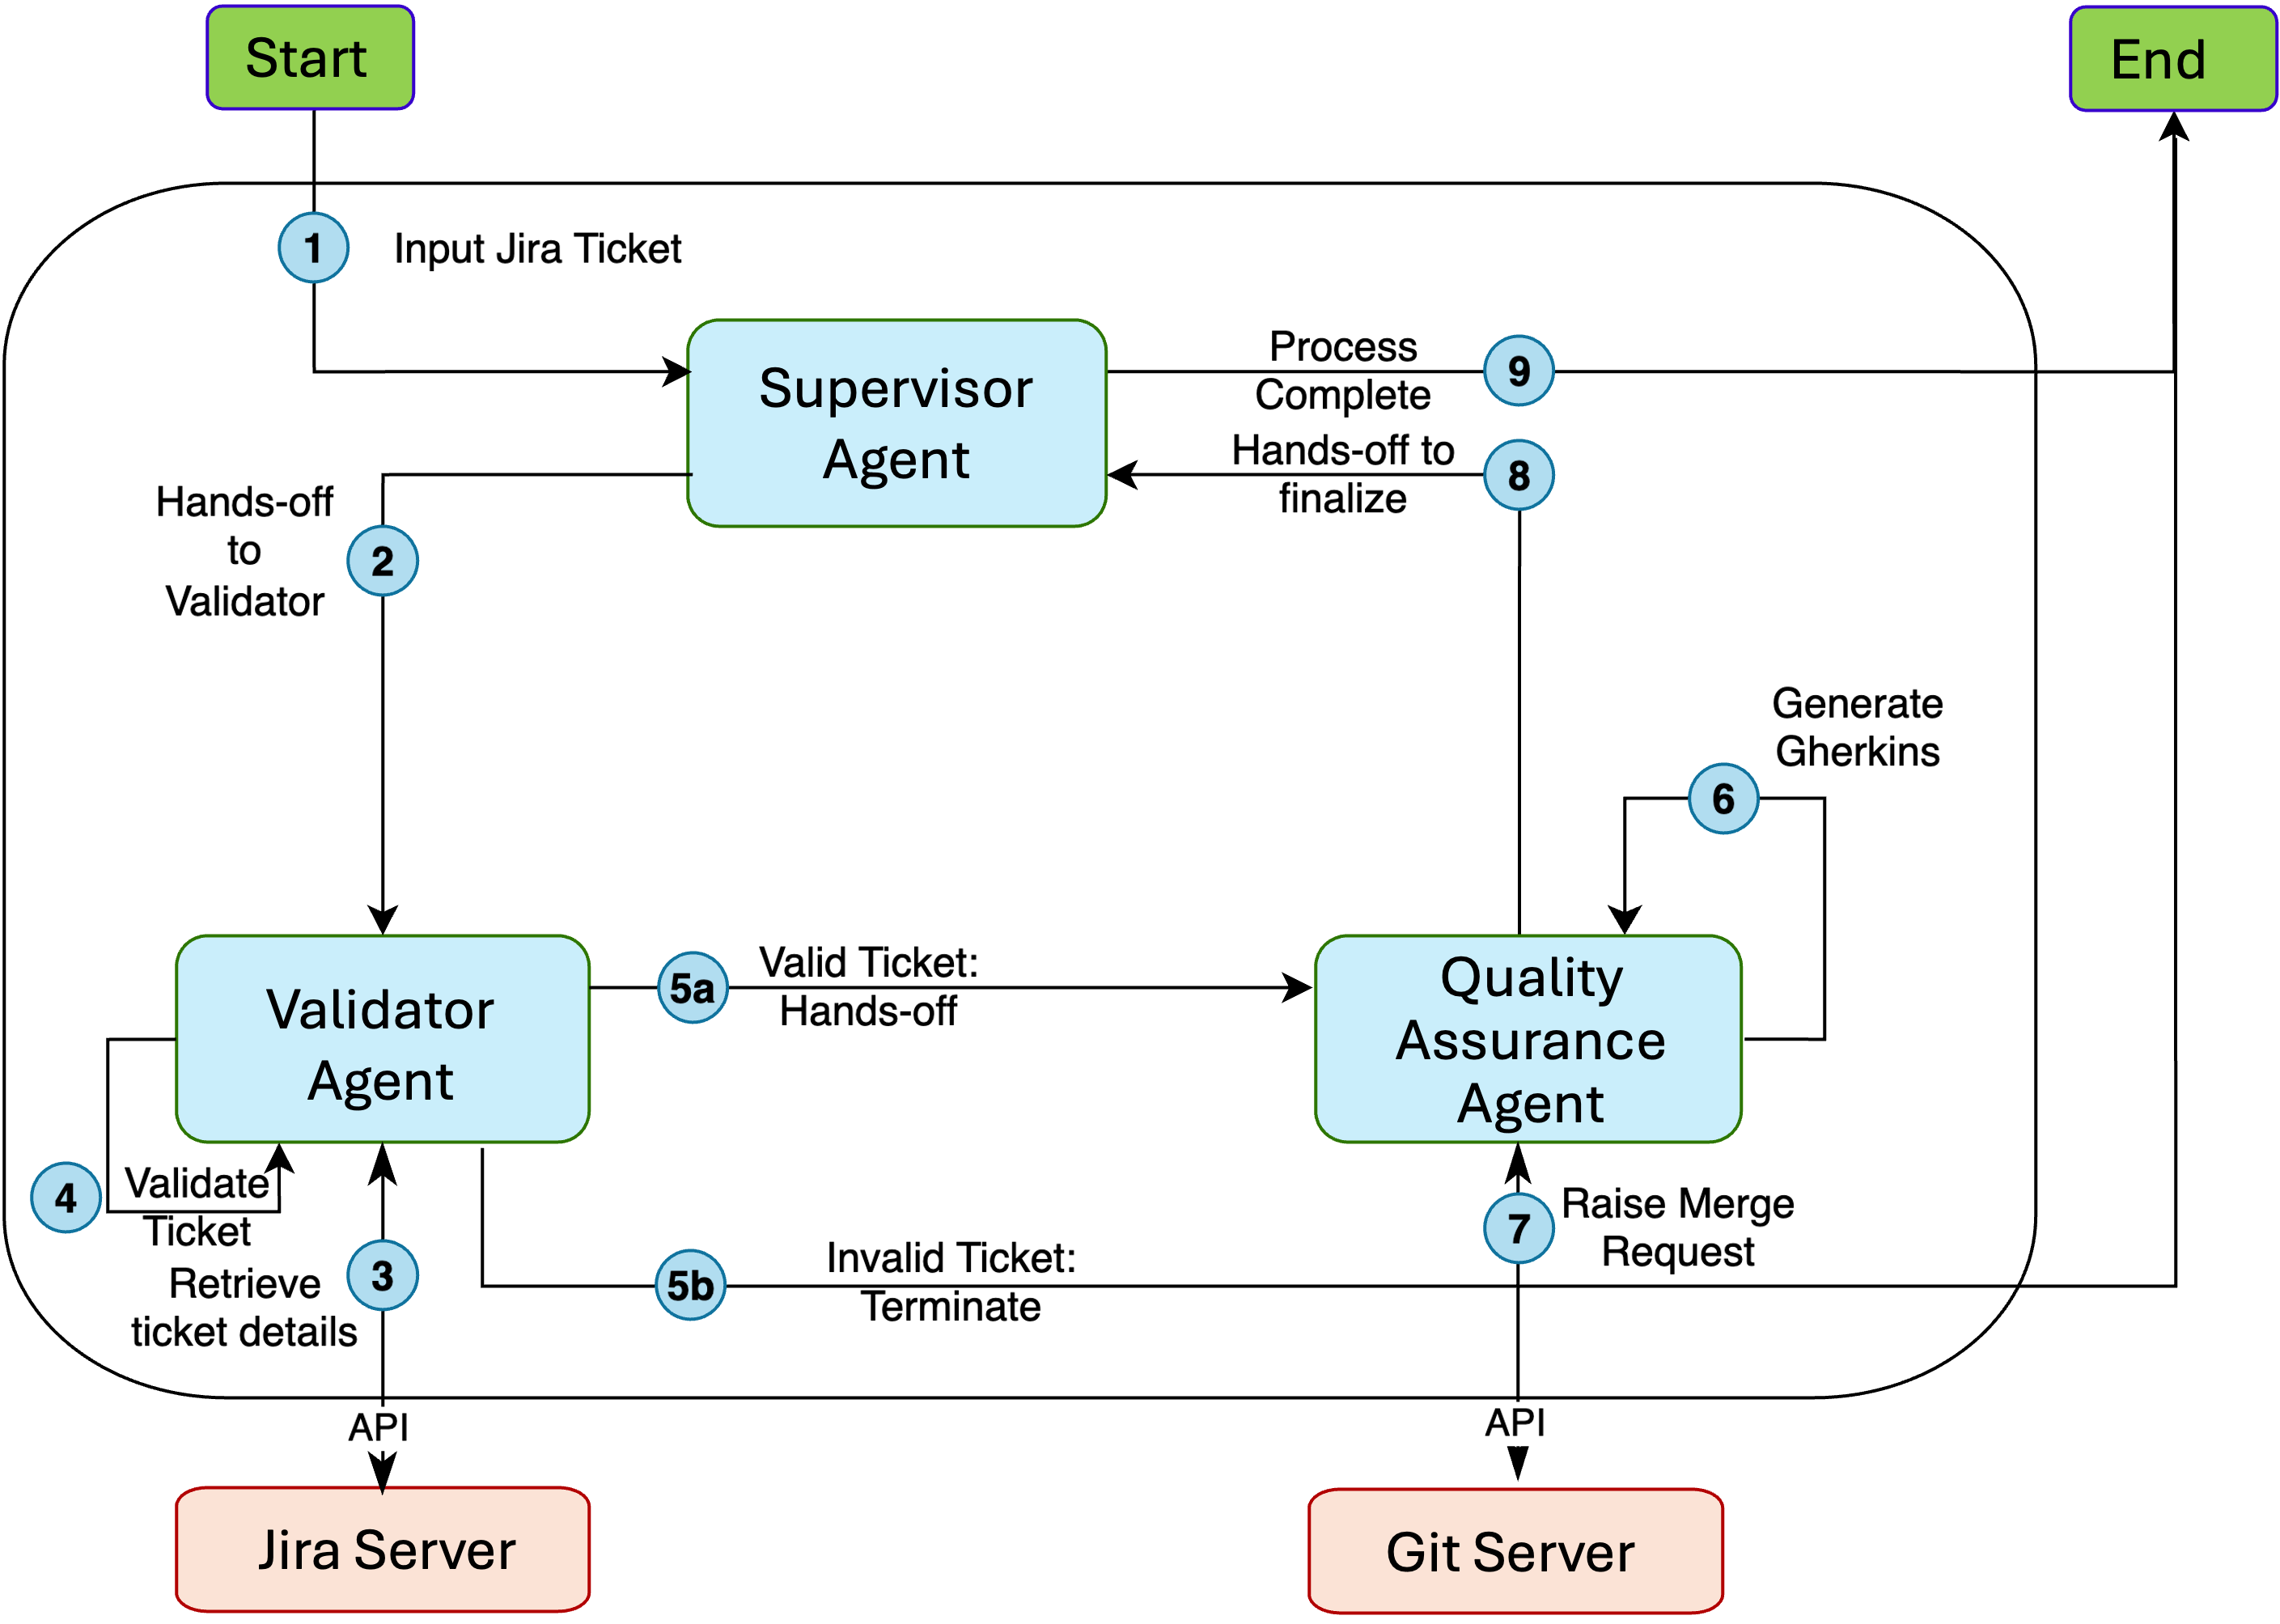
\includegraphics[width=\linewidth]{figures/architecture-v5.png}
\caption{Architecture and operational workflow of CMAS4G2. The diagram illustrates the nine-step process involving the Supervisor, Validator, and Quality Assurance agents.}
\label{fig:MAS-design}
\end{figure}

CMAS4G2 leverages Microsoft's AutoGen Swarm framework to orchestrate interactions among three specialized agents:

\begin{itemize}[leftmargin=*]
    \item \textbf{Supervisor Agent:} Acts as the central orchestration component, managing workflow execution and ensuring correct handoffs between specialized agents.
    \item \textbf{Validator Agent:} Focuses on Jira ticket analysis and content validation. This agent establishes direct API connectivity with Jira to retrieve ticket data and perform systematic validation checks.
    \item \textbf{Quality Assurance Agent:} Transforms validated requirements into executable Gherkin acceptance tests, combining domain knowledge in test design patterns with automated code generation capabilities.
\end{itemize}

The end-to-end workflow proceeds through the following phases:

\begin{enumerate}[leftmargin=*]
    \item \textbf{Initialization Phase:} The Supervisor Agent receives the input Jira ticket and orchestrates its handoff to the Validator Agent.
    \item \textbf{Validation Phase:} The Validator Agent retrieves ticket details via the Jira API and performs content validation. Tickets that fail validation are rejected with documented deficiencies.
    \item \textbf{Generation Phase:} Upon successful validation, the Quality Assurance Agent generates Gherkin test scripts and creates automated merge requests in Git.
    \item \textbf{Completion Phase:} The Supervisor Agent manages the final coordination steps and concludes the workflow.
\end{enumerate}

\subsection{Evaluation Framework}

We employ the LLM-as-a-Judge (LAJ) framework from Section~\ref{sec:llm_judge} for evaluating generated Gherkin scripts, using GPT-4o Mini as the judge model following calibration against expert human annotations. This integration demonstrates the practical utility of the LAJ framework for downstream agentic applications.

\subsubsection{Dataset}

The benchmark comprises 200 synthetic Jira tickets based on the open-source Kill Bill subscription billing platform:
\begin{itemize}[leftmargin=*]
    \item \textbf{Valid Tickets (IDs 1--100):} Complete tickets for successful Gherkin generation
    \item \textbf{Invalid Tickets (IDs 101--200):} Deliberately incomplete tickets to test rejection logic
\end{itemize}

\subsubsection{Performance Metrics}

\begin{itemize}[leftmargin=*]
    \item \textbf{Valid Ticket Success Rate:} Percentage of well-formed tickets for which the system successfully generates Gherkin scripts
    \item \textbf{Invalid Ticket Success Rate:} Percentage of incomplete tickets correctly rejected before test generation
    \item \textbf{Overall Success Rate:} Combined success: (Valid SR + Invalid SR)/2
    \item \textbf{Average Test Coverage:} Mean coverage score assigned by the LAJ framework
\end{itemize}

\subsection{Results}

Table~\ref{tab:cmas4g2_results} presents performance across model configurations.

\begin{table}[htbp]
\centering
\caption{CMAS4G2 Performance on 200-Ticket Kill Bill Benchmark. Values are mean$\pm$std across 5 runs.}
\label{tab:cmas4g2_results}
\resizebox{\textwidth}{!}{%
\begin{tabular}{@{}llcccc@{}}
\toprule
\textbf{Model} & \textbf{Config} & \textbf{Valid (\%)} & \textbf{Invalid (\%)} & \textbf{Overall (\%)} & \textbf{Coverage (\%)} \\
\midrule
Claude Sonnet 4 & -- & \textbf{100.0$\pm$0} & \textbf{80.8$\pm$0} & \textbf{90.4$\pm$0} & \textbf{91.6$\pm$0} \\
\midrule
\multirow{2}{*}{GPT-OSS 20B} & medium & 99.2$\pm$2 & 76.0$\pm$0 & 87.6$\pm$1 & 85.4$\pm$0 \\
 & high & 1.6$\pm$3 & 73.0$\pm$0 & 37.3$\pm$2 & 16.8$\pm$34 \\
\midrule
\multirow{2}{*}{Qwen3-32B} & no think & 99.2$\pm$1 & 35.2$\pm$0 & 67.2$\pm$1 & 86.9$\pm$0 \\
 & think & 87.2$\pm$5 & 69.0$\pm$0 & 78.1$\pm$2 & 83.7$\pm$0 \\
\midrule
\multirow{2}{*}{Qwen3-8B} & no think & 58.8$\pm$24 & 41.0$\pm$0 & 49.9$\pm$12 & 79.5$\pm$3 \\
 & think & 98.0$\pm$2 & 57.0$\pm$0 & 77.5$\pm$1 & 79.2$\pm$0 \\
\bottomrule
\end{tabular}
}
\end{table}

\subsubsection{Key Findings}

\textbf{Open-Weight Models Approach Proprietary Performance.} GPT-OSS 20B (medium) achieves 87.6\% overall success and 85.4\% coverage, approaching within 2.8 percentage points of Claude Sonnet 4's 90.4\% and 91.6\% while enabling fully local deployment.

\textbf{Reasoning Configuration Critically Affects Quality.} The impact of reasoning mode varies dramatically by model size:
\begin{itemize}[leftmargin=*]
    \item \textbf{Small models benefit dramatically:} Qwen3-8B improves from 49.9\% to 77.5\% overall success with thinking mode---a 27.6 percentage point gain
    \item \textbf{Large models show mixed effects:} Qwen3-32B degrades from 99.2\% to 87.2\% valid ticket success with thinking mode, while improving invalid ticket rejection from 35.2\% to 69.0\%
    \item \textbf{Excessive reasoning causes catastrophic failure:} GPT-OSS 20B (high) collapses to 1.6\% valid success due to context exhaustion before completing Gherkin generation
\end{itemize}

These reasoning configuration findings directly inform Chapter~\ref{ch:strategies}, where we systematically characterize the relationship between reasoning intensity and task complexity across sentiment analysis tasks.

\textbf{Invalid Ticket Rejection Remains Challenging.} All models struggle with invalid ticket rejection compared to valid ticket processing. Claude Sonnet 4 achieves only 80.8\% rejection rate, with open-weight models ranging from 35.2\% to 76.0\%. This asymmetry suggests that correctly identifying \textit{missing} information is harder than processing \textit{present} information.

\subsection{Integration Summary}

The successful integration of CMAS4G2 with the LAJ framework demonstrates the practical value of our multi-dimensional evaluation approach. By establishing ECR@1 and adjusted cost metrics in Section~\ref{sec:llm_judge}, we enabled reliable, cost-effective evaluation of generated tests at scale---a critical capability for operationalizing automated test generation in enterprise CI/CD pipelines.

%% =============================================================================
%% PART 3: Standalone Systems (Papers 5-6)
%% =============================================================================

\section{Hierarchical Multi-Agent System for Payments}
\label{sec:hmasp}

While the preceding sections focus on back-office automation and software quality assurance, payment processing presents distinct challenges: traditional payment infrastructure employs anti-bot mechanisms, multi-factor authentication, and fraud detection systems that constrain agentic technology adoption. This section presents HMASP (Hierarchical Multi-Agent System for Payments)~\cite{huang2026hmasp}, the first LLM-based multi-agent system to implement end-to-end agentic payment workflows.

\subsection{Architecture Overview}

HMASP addresses end-to-end agentic payment processing through a modular, four-level hierarchical design implemented using LangGraph~\cite{langchain2024langgraph}. Figure~\ref{fig:MAS-design} illustrates the architecture.

\begin{figure}[!h]
    \centering
    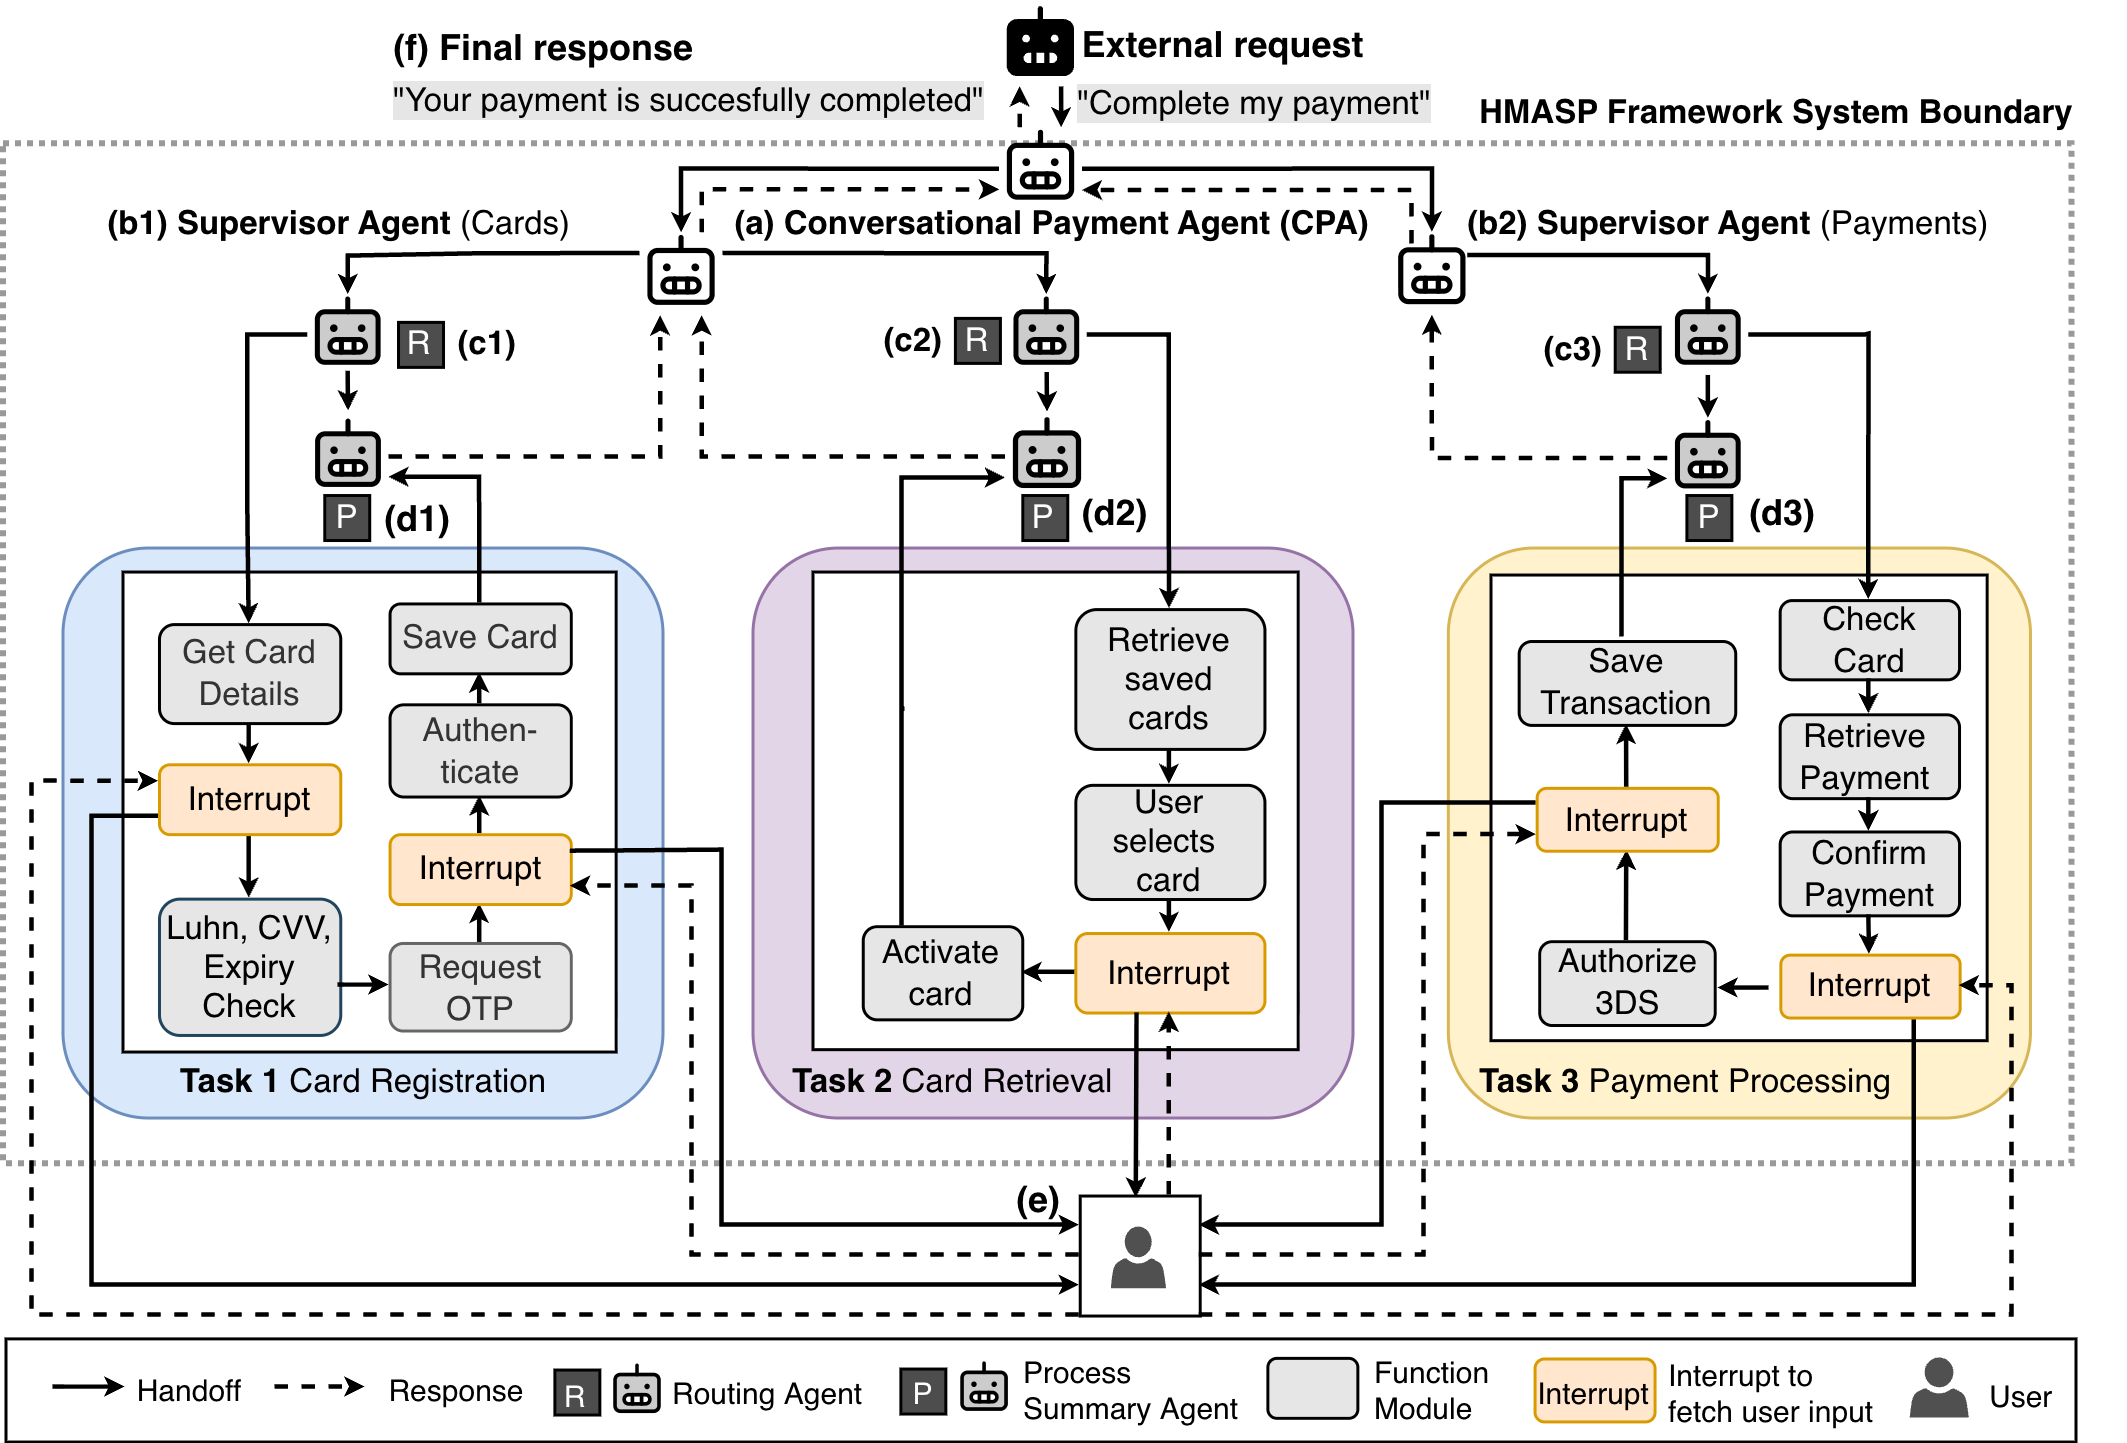
\includegraphics[width=\textwidth]{figures/ConvPayAgent6.png}
    \caption{Overview of the proposed HMASP. An external request (e.g., ``Complete my payment'') is sent to the Conversational Payment Agent (CPA - first agent level);
    (a) The CPA processes the request and delegates it to one of the two Supervisors (b1, b2 - second agent level) for further handling;
    (b) The selected Supervisor routes the request to a suitable Routing agent (c1, c2, or c3 - third agent level);
    (c) Routing agents initiate the corresponding task-specific workflow (Task 1, Task 2, Task 3);
    Upon initiation, a series of task-relevant function modules are triggered to complete the request;
    (d) Upon task completion, the Process summary agent (d1, d2, d3 - fourth agent level) compiles the outcome and generates a response. This summary response is propagated upward the system hierarchy through Supervisor agents and CPA;
    (e) When user input is required to complete the task, an interrupt mechanism is triggered to obtain the necessary input before execution resumes;
    (f) Finally, the CPA responds to the request (e.g., ``Your payment has been successfully completed'').
    }
    \label{fig:MAS-design}
\end{figure}

\subsubsection{Agent Hierarchy}

The hierarchy comprises four distinct agent levels:

\begin{enumerate}[leftmargin=*]
    \item \textbf{Conversational Payment Agent (CPA):} Primary orchestrator receiving external requests. The CPA handles all incoming requests and coordinates task delegation to supervisors. It can also reject irrelevant requests.
    
    \item \textbf{Supervisor Agents:} Decision-makers that delegate requests based on context and workload to appropriate sub-workflows. Each supervisor is responsible for reporting outcomes back to the CPA.
    
    \item \textbf{Routing Agents:} Identify and initiate task-specific workflows. They serve as the final decision layer on whether to trigger payment-related function modules or reject irrelevant requests.
    
    \item \textbf{Process Summary Agents:} Interact with underlying systems to execute operations and generate structured responses on workflow outcomes.
\end{enumerate}

\subsubsection{Architectural Patterns}

HMASP incorporates several architectural patterns ensuring reliable payment processing:

\textbf{Shared State Variables:} Graph States consist of user-defined variables that persist throughout MAS runtime. Agents can only access their assigned states, preventing unauthorized read/write across state variables.

\textbf{Information Determinism:} Critical payment information is stored in state variables rather than generated by LLMs. This decouples payment-related processing from generative processes---payment amounts, card numbers, and transaction IDs are retrieved from state variables, never hallucinated.

\textbf{Structured Handoffs:} Agents use LangGraph's handoff mechanism to seamlessly pass processes to one another, enabling coordination where requests flow from CPA through the hierarchy.

\textbf{Interrupt Mechanism:} When user input is required during execution (e.g., OTP verification, card selection), an interrupt mechanism pauses the workflow to collect necessary input before proceeding.

\subsection{Evaluation}

We constructed a dataset of 1,000 payment-related inputs across four task categories: Card Registration (250), Card Retrieval (250), Payment Checkout (250), and Irrelevant Inputs (250).

\subsection{Results}

Table~\ref{tab:hmasp_results} presents task success rates across models.

\begin{table}[htbp]
\centering
\caption{HMASP Task Success Rates (\%) Across Models}
\label{tab:hmasp_results}
\begin{tabular}{@{}lcccc@{}}
\toprule
\textbf{Model} & \textbf{Task 1} & \textbf{Task 2} & \textbf{Task 3} & \textbf{Task 4} \\
\midrule
GPT-4.1 (Baseline) & \textbf{99.6} & \textbf{99.6} & \textbf{99.6} & \textbf{100.0} \\
Qwen2.5:32b & 97.2 & 98.4 & 98.8 & 100.0 \\
Qwen2.5:14b & 94.0 & 95.2 & 98.8 & 100.0 \\
Qwen3:32b & 99.6 & 35.2 & 39.6 & 100.0 \\
Mistral-small3.2:24b & 94.8 & 94.0 & 82.8 & 100.0 \\
Llama3.1:70b & 87.2 & 88.4 & 47.2 & 33.2 \\
Llama3.1:8b & 38.0 & 38.4 & 39.2 & 3.6 \\
\bottomrule
\end{tabular}
\end{table}

\subsubsection{Key Findings}

\textbf{Open-Source Viability:} Qwen2.5:32b achieves an average 97.0\% task success rate across payment-relevant tasks (Tasks 1--3), demonstrating viability for end-to-end agentic payments with open-weight models.

\textbf{Inconsistent Performance Across Tasks:} Some models show inconsistent behavior---Qwen3:32b achieves 99.6\% on Task 1 but only 35.2\% and 39.6\% on Tasks 2 and 3, indicating that strong performance on one task does not guarantee reliability across the workflow.

\textbf{Irrelevant Input Handling:} Most models correctly reject irrelevant inputs (Task 4), with Qwen2.5 variants achieving 100\%. However, Llama3.1 models showed weakness, with Llama3.1:8b achieving only 3.6\%.

\subsection{Novelty and Contributions}

To our knowledge, HMASP is the first LLM-based multi-agent system supporting fully end-to-end agentic payment workflows. Table~\ref{tab:comparative-study-table} provides comparative analysis with existing approaches.

\begin{table}[!h]
  \centering
  \begin{threeparttable}
  \begin{tabular}{
      p{0.18\linewidth}%
      >{\centering\arraybackslash}p{0.10\linewidth}%
      >{\centering\arraybackslash}p{0.12\linewidth}%
      >{\centering\arraybackslash}p{0.12\linewidth}%
      >{\centering\arraybackslash}p{0.15\linewidth}%
      >{\centering\arraybackslash}p{0.12\linewidth}
    }
    \toprule
    \textbf{Method} & \textbf{Open-Weight LLM} & \textbf{Full Payment Processing} & \textbf{TR Success Rate (\%)} & \textbf{TR Precision-Recall (\%)} & \textbf{TR F1-Score (\%)} \\
    \midrule
    LLMPA~\cite{guan2024llmprocessautomation} & Yes & No\tnote{1} & 76.5 & -- & -- \\
    Method 1~\cite{dahiphale2024llmscampayments} & No & No & 93.3 & 85.7--30.2 & 44.77 \\
    Method 2~\cite{qu-etal-2025-llm-fraud} & Yes & No & -- & N/A\tnote{2}--73.7 & -- \\
    \midrule
    \textbf{HMASP (Ours)} & \textbf{Yes} & \textbf{Yes} & \textbf{97.7} & \textbf{99.4--98.8} & \textbf{99.2} \\
    \bottomrule
  \end{tabular}
  \begin{tablenotes}
    \small
    \item[1] Processing stops at network boundary; defaults to in-app checkout.
    \item[2] Not reported.
  \end{tablenotes}
  \caption{A comparative overview of existing autonomous agents in payment-relevant processes with their Task-Relevant (TR) metrics. For HMASP, averages from the best-performing open-weight LLM (Qwen2.5:32b) were reported.}
  \label{tab:comparative-study-table}
  \end{threeparttable}
\end{table}

%% =============================================================================
%% Section: EdgeAgent - Semi-Automatic Annotation Pipeline
%% =============================================================================

\section{EdgeAgent and Agentic Success Rate: Semi-Automatic Annotation with Reliability Metrics}
\label{sec:edgeagent}

This section presents EdgeAgent~\cite{huang2026edgeagent}---a semi-automatic data labeling pipeline that orchestrates tool-using LLMs on edge devices for specialized domain annotation. A central contribution is the \textbf{Agentic Success Rate (ASR)} metric, which provides fine-grained evaluation of tool-calling precision throughout multi-step workflows, complementing the 12-category error taxonomy introduced in Section~\ref{sec:diagnostic_framework}. Using maritime risk assessment as a case study, we evaluate 14 open-source Qwen models (0.5B--72B) against GPT-4.1 variants across three hardware platforms, demonstrating that open-source models can achieve production-quality annotation while preserving privacy.

\subsection{Motivation}

Data labeling and annotation constitute critical bottlenecks in machine learning pipelines, particularly for specialized domains requiring expert knowledge~\cite{huang2024automating}. Maritime risk assessment exemplifies these challenges: incidents span diverse categories (weather events, accidents, cyber attacks, administrative issues), require domain expertise to classify correctly, and emerge continuously from news sources worldwide. Traditional manual annotation approaches are labor-intensive, expensive, and struggle to scale with the volume and velocity of incoming data.

Privacy concerns may prohibit sending sensitive data to cloud APIs, latency requirements demand local processing, and resource constraints on edge devices limit model selection. Furthermore, annotation pipelines require more than classification---they need tool integration for data retrieval, content extraction, multi-step reasoning, and database operations.

\subsection{Semi-Automatic Labeling Pipeline Architecture}

The EdgeAgent pipeline implements an interactive workflow where researchers submit URLs of news articles and receive automated annotations through LLM-orchestrated tool calls. Figure~\ref{fig:edgeagent_architecture} illustrates the architecture.

\begin{figure}[htbp]
    \centering
    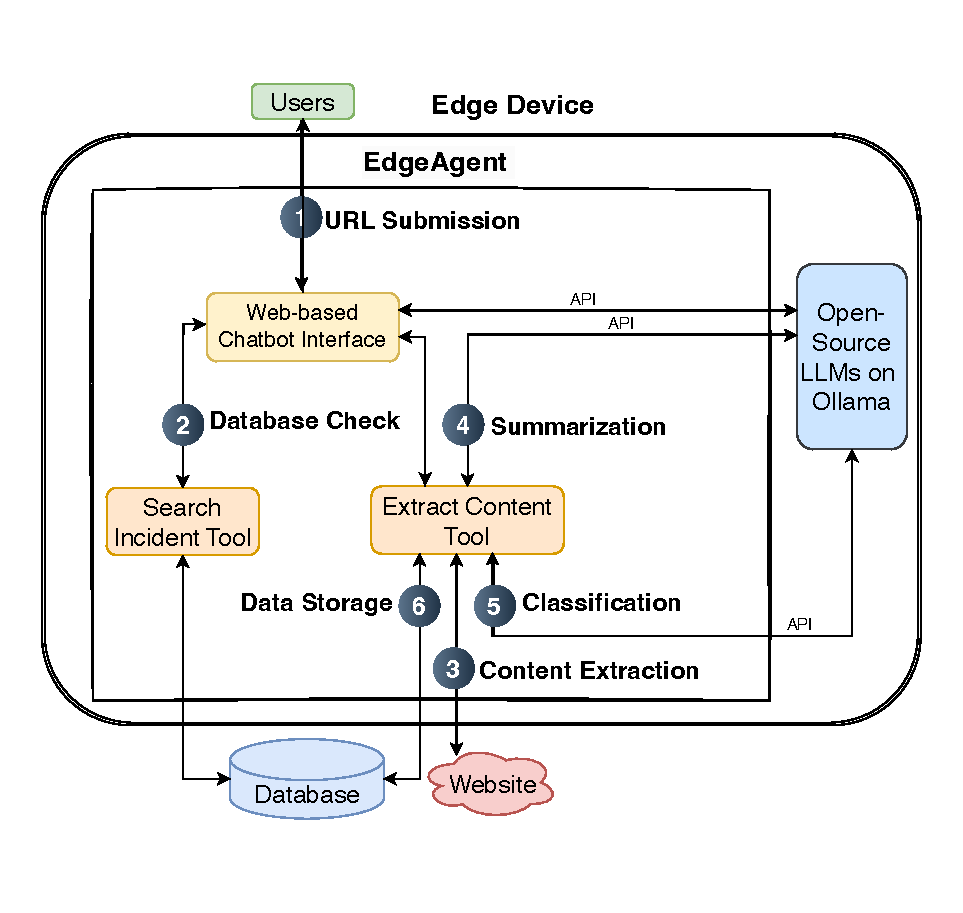
\includegraphics[width=\textwidth]{images/Edge_AI_Agents_v5.drawio.pdf}
    \caption{EdgeAgent Architecture: Semi-Automatic Data Labeling Pipeline. The system orchestrates LLM-powered agents for (1) URL submission, (2) database checking, (3) content extraction, (4) summarization, (5) classification, and (6) data storage. Open-source LLMs run locally on edge devices, enabling privacy-preserving annotation without cloud dependency.}
    \label{fig:edgeagent_architecture}
\end{figure}

The semi-automatic workflow consists of six key steps:

\begin{enumerate}[leftmargin=*]
    \item \textbf{URL Submission:} Researchers submit URLs through a web-based interface, initiating the annotation process.
    \item \textbf{Database Check:} EdgeAgent queries the database to avoid duplicate labeling, retrieving existing annotations if available.
    \item \textbf{Content Extraction:} An integrated tool extracts textual content from submitted URLs, handling diverse web formats.
    \item \textbf{Summarization:} Selected LLMs generate concise summaries emphasizing incident details, location, and consequences.
    \item \textbf{Classification:} LLMs classify summarized content into predefined risk categories using few-shot prompting.
    \item \textbf{Data Storage and Retrieval:} Annotated data is stored in a structured database, enabling interactive queries and visualization.
\end{enumerate}

Beyond automated annotation, EdgeAgent's agentic architecture enables researchers to interactively query the accumulated database using natural language and manually update labels when automated classifications require refinement.

\subsection{Agentic Success Rate: Evaluating Annotation Pipeline Reliability}

In automated labeling systems, LLMs must correctly orchestrate multiple tools across workflow steps. Traditional binary metrics (task success/failure) can mask partial failures where some annotation steps succeed while others fail. To address this limitation, we introduce the \textbf{Agentic Success Rate (ASR)}---a fine-grained metric quantifying tool-calling precision throughout multi-step workflows.

\subsubsection{Metric Definition}

We formalize ASR by decomposing agentic workflows into atomic evaluation steps. For a pipeline with $n$ evaluable steps, let $S_i \in \{0, 1\}$ indicate successful completion of step $i$. The Overall Agentic Score (OAS) aggregates these indicators:

\begin{equation}
\text{OAS} = \sum_{i=1}^{n} w_i \cdot S_i
\end{equation}

where $w_i$ represents developer-defined weights (default: 1). The Agentic Success Rate normalizes this score:

\begin{equation}
\text{ASR} = \frac{\text{OAS}}{\sum_{i=1}^{n} w_i}
\end{equation}

An ASR of 1.00 (100\%) indicates flawless pipeline execution; lower scores pinpoint specific failure modes. For example, a model correctly invoking both tools but mishandling URL transmission at step $S_5$ yields OAS=4, ASR=0.57---revealing partial success that binary metrics would score as complete failure.

\subsubsection{Generality of the Framework}

Although demonstrated with maritime annotation, ASR applies to arbitrary agentic architectures. In general, agent execution forms a directed acyclic graph (DAG) where internal nodes represent reasoning states and leaf nodes are tool calls. During execution, the LLM traverses a path through this DAG, with each edge terminating in one or more tool invocations.

Because dispatch logic is developer-controlled, every call and sub-step can be logged, time-stamped, and scored at arbitrary granularity. The framework is computed by:
\begin{enumerate}[leftmargin=*]
    \item Enumerating evaluable sub-steps along the observed traversal
    \item Assigning developer-defined weights and error categories
    \item Normalizing by the path's maximum attainable score
\end{enumerate}

This design enables consistent evaluation across chains, trees, or complex DAGs while preserving step-level diagnostics comparable across diverse architectures and domains.

\subsubsection{Application to EdgeAgent}

The EdgeAgent pipeline employs two tools: \texttt{search\_incident} (database lookup) and \texttt{extract\_content} (web scraping). We decompose each labeling task into seven atomic steps ($S_i$, where $i = 1, 2, \ldots, 7$):

\begin{itemize}[leftmargin=*]
    \item[$S_1$] Invocation of \texttt{search\_incident}
    \item[$S_2$] Transmission of the URL parameter to \texttt{search\_incident}
    \item[$S_3$] Execution of the database query
    \item[$S_4$] Invocation of \texttt{extract\_content}
    \item[$S_5$] Transmission of the URL parameter to \texttt{extract\_content}
    \item[$S_6$] Completion of summarization
    \item[$S_7$] Completion of classification (label generation)
\end{itemize}

The stepwise breakdown provides actionable insights for improving labeling pipelines. Tool invocation failures ($S_1$, $S_4$) indicate prompt engineering issues or insufficient model capacity for structured workflows. Parameter transmission errors ($S_2$, $S_5$) reveal hallucination problems where models generate invalid tool arguments. Processing failures ($S_6$, $S_7$) suggest downstream component issues or data quality problems. This granularity guides targeted improvements, distinguishing orchestration failures (fixable through better prompting) from fundamental model limitations (requiring larger models).

\subsection{Experimental Setup}

\paragraph{Model Integration.} We evaluate OpenAI models (GPT-4.1-nano, GPT-4.1-mini, GPT-4.1) and open-source models (Qwen 2.5: 0.5B--72B, Qwen 3: 0.6B--32B). Qwen3 models support dual-mode reasoning: thinking mode enables complex multi-step reasoning, while non-thinking mode provides rapid responses.

\paragraph{Dataset.} We collected 2,232 maritime news articles, curating 1,003 articles for evaluation after filtering. Ground truth labels were obtained with GPT-4o and refined through human review.

\paragraph{Hardware Configurations.} Testing across three platforms: NVIDIA H100 (enterprise), NVIDIA RTX 4090 (consumer GPU), and Apple M3 Max (portable edge device).

\subsection{Results}

Table~\ref{tab:edgeagent_results_full} presents comprehensive evaluation results.

\begin{table}[htbp]
\centering
\caption{EdgeAgent Model Performance for Semi-Automatic Data Labeling. For Qwen3 models, (T) denotes thinking mode and (N) denotes standard mode. All Qwen results obtained on H100 platform.}
\label{tab:edgeagent_results_full}
\begin{tabular}{@{}lcccc@{}}
\toprule
\textbf{Model} & \textbf{ASR (\%)} & \textbf{TSR (\%)} & \textbf{F1 (\%)} & \textbf{MRT (s)} \\
\midrule
\multicolumn{5}{l}{\textit{Qwen Models (Selected)}} \\
qwen2.5:7b & 74.48 & 60.32 & 81.88 & 12.8 \\
qwen2.5:14b & 76.88 & 75.57 & 83.38 & 15.3 \\
qwen2.5:32b & 93.36 & 93.32 & 82.45 & 15.1 \\
qwen2.5:72b & 94.99 & 93.12 & \textbf{86.19} & 38.7 \\
qwen3:32b (T) & \textbf{98.21} & \textbf{97.21} & 82.98 & 36.0 \\
qwen3:32b (N) & 84.29 & 74.88 & 83.17 & 28.9 \\
\midrule
\multicolumn{5}{l}{\textit{OpenAI Models}} \\
GPT-4.1-nano & 98.08 & 99.40 & 65.55 & \textbf{7.3} \\
GPT-4.1-mini & 99.49 & 99.60 & \textbf{86.17} & 13.4 \\
GPT-4.1 & \textbf{99.91} & \textbf{100.00} & 83.61 & 14.1 \\
\bottomrule
\end{tabular}
\end{table}

\subsubsection{Key Findings}

\textbf{Open-Source Models Match Proprietary Quality.} qwen3:32b (T) achieves 98.21\% ASR, 97.21\% TSR, and 82.98\% F1---performance nearly matching GPT-4.1. This demonstrates that local, privacy-preserving annotation pipelines can deliver quality comparable to cloud-based proprietary alternatives.

\textbf{Model Size Determines Annotation Reliability.} Smaller models ($<$4B) exhibit significant disparities between task completion and proper workflow execution. For example, qwen3:0.6b achieves 84.35\% TSR but only 0.10\% ASR, indicating it bypasses required database lookup steps rather than following proper annotation protocols.

\textbf{Thinking Mode Enhances Multi-Step Annotation.} qwen3:32b (T) achieves 98.21\% ASR compared to 84.29\% in non-thinking mode---a 14-point difference demonstrating the value of extended reasoning for complex workflows. This finding connects directly to the reasoning configuration analysis in Chapter~\ref{ch:strategies}, where we characterize the Reasoning Intensity (RI) metric and its relationship to task complexity.

\textbf{Annotation Quality is Hardware-Independent.} All platforms exhibit consistent ASR and TSR patterns across models. Model selection governs annotation quality, while hardware determines throughput. qwen2.5:32b completes tasks in 15s on H100, compared to 169s on RTX 4090 and 296s on M3 Max---representing 11.3$\times$ and 19.7$\times$ speedups respectively.

\subsection{Diagnostic Value and Cross-Domain Applicability}

The ASR metric and its application to EdgeAgent validate the cross-domain applicability of fine-grained reliability evaluation. The same diagnostic principles apply across domains:

\begin{itemize}[leftmargin=*]
    \item Tool-calling errors dominate failures for smaller models
    \item Processing quality remains consistent once workflows are properly initiated
    \item The three-tier deployment guidance (${<}$4B unsuitable, 7B--14B transitional, ${\geq}$32B production-ready) generalizes across applications
\end{itemize}

Combined with the 12-category error taxonomy from Section~\ref{sec:diagnostic_framework}, ASR provides comprehensive diagnostics for multi-agent LLM systems---enabling practitioners to systematically diagnose failure modes and guide targeted improvements.

%% =============================================================================
%% Practical Guidelines and Summary
%% =============================================================================

\section{Practical Deployment Guidelines}
\label{sec:agentic_guidelines}

Based on our research across six systems, we provide consolidated guidelines for enterprise agentic AI deployment:

\subsection{Architecture Design}

\begin{enumerate}[leftmargin=*]
    \item \textbf{Modular agent specialization:} Design agents with clearly defined, focused responsibilities
    \item \textbf{Hierarchical coordination:} Employ multi-level hierarchies for complex workflows, enabling modular task execution
    \item \textbf{Information determinism:} Store critical information in state variables, not LLM outputs, preventing hallucination of sensitive data
    \item \textbf{Structured handoffs:} Implement clear protocols for inter-agent communication
    \item \textbf{Human oversight:} Incorporate validation checkpoints for high-impact decisions
\end{enumerate}

\subsection{Model Selection}

\begin{enumerate}[leftmargin=*]
    \item \textbf{Large models ($\geq$32B):} Provide production-ready reliability (ASR $>$93\%) for autonomous workflows
    \item \textbf{Mid-tier models (7B--14B):} Suitable for interactive workflows with human review, balancing accuracy and latency
    \item \textbf{Small models ($<$4B):} Unsuitable for multi-step agentic pipelines despite acceptable performance on isolated tasks
    \item \textbf{Consider edge deployment:} Reduces latency, improves privacy, and eliminates API costs---qwen2.5:32b matches proprietary performance while enabling local deployment
\end{enumerate}

\subsection{Reliability Engineering}

\begin{enumerate}[leftmargin=*]
    \item \textbf{Measure ECR@1:} Always capture first-attempt success rates alongside accuracy
    \item \textbf{Implement retry logic:} Budget 5--15\% overhead for reliability failures
    \item \textbf{Monitor operational metrics:} Track ECR@1, latency, and cost in production
    \item \textbf{Use adjusted cost metrics:} Account for retry overhead in total cost of ownership
\end{enumerate}

\subsection{Evaluation Strategy}

\begin{enumerate}[leftmargin=*]
    \item \textbf{Use fine-grained metrics:} Adopt ASR or similar stepwise metrics to diagnose failure modes beyond binary success/failure
    \item \textbf{Distinguish orchestration from processing:} Tool-calling failures require different interventions than classification errors
    \item \textbf{Hardware-aware benchmarking:} Test on target deployment hardware to establish realistic performance expectations
    \item \textbf{Multi-dimensional evaluation:} Assess accuracy, reliability, and cost together for production readiness
\end{enumerate}

\section{Summary}
\label{sec:agentic_summary}

This chapter demonstrated the viability and effectiveness of agentic AI for automating complex enterprise workflows, addressing the second research question (RQ2) on designing and evaluating multi-agent LLM systems for reliable, scalable enterprise automation. Key contributions include:

\begin{enumerate}[leftmargin=*]
    \item \textbf{Multi-agent invoice reconciliation (Section~\ref{sec:invoice_reconciliation}):} Validated architecture achieving 99.9\% success rate with edge-deployed open-source models, demonstrating that qwen2.5:32b outperforms proprietary alternatives while consuming only 523J per task on consumer hardware
    
    \item \textbf{Diagnostic framework for tool invocation reliability (Section~\ref{sec:diagnostic_framework}):} Novel 12-category error taxonomy providing systematic failure characterization for multi-agent systems, distinguishing tool initialization, parameter handling, execution, and result interpretation errors
    
    \item \textbf{LLM-as-Judge framework with ECR@1 (Section~\ref{sec:llm_judge}):} Production-ready evaluation system introducing Evaluation Completion Rate to capture operational reliability, revealing 175$\times$ cost variation and demonstrating that GPT-4o Mini achieves best-in-class accuracy at 78$\times$ cost reduction versus premium models
    
    \item \textbf{CMAS4G2 for acceptance test generation (Section~\ref{sec:cmas4g2}):} Cooperative multi-agent system leveraging the LLM-as-Judge framework, demonstrating that open-weight models (GPT-OSS 20B: 87.6\% success) approach proprietary performance (Claude Sonnet 4: 90.4\%) while revealing critical reasoning configuration trade-offs
    
    \item \textbf{Hierarchical Multi-Agent System for Payments (Section~\ref{sec:hmasp}):} First LLM-based multi-agent system implementing end-to-end agentic payment workflows, achieving 97.0\% task success rate with architectural patterns enabling modular payment processing
    
    \item \textbf{EdgeAgent and Agentic Success Rate (Section~\ref{sec:edgeagent}):} Semi-automatic annotation pipeline introducing the ASR metric for fine-grained reliability evaluation, with qwen3:32b achieving 98\% ASR and 83\% F1 matching GPT-4.1 quality while enabling privacy-preserving edge deployment
\end{enumerate}

The ASR and ECR@1 metrics represent methodological contributions with broad applicability, extending the multi-dimensional evaluation philosophy established with RAP in Chapter~\ref{ch:rag}. ASR, introduced in Section~\ref{sec:edgeagent}, decomposes agentic workflows into atomic steps, enabling practitioners to systematically diagnose failure modes and guide targeted improvements. Combined with the 12-category error taxonomy from Section~\ref{sec:diagnostic_framework}, these tools provide comprehensive diagnostics for multi-agent systems. ECR@1 captures operational reliability invisible to accuracy-only evaluation, revealing cost implications crucial for production deployment. Together, these metrics complement traditional accuracy measures and enable meaningful comparison across diverse agentic architectures.

A consistent theme across all six systems is the viability of open-source models for enterprise deployment. qwen2.5:32b matches GPT-4.1 performance across invoice reconciliation (100\% vs 100\%), payment processing (97.0\% average), and annotation (93.36\% ASR) while enabling privacy-preserving edge deployment. This finding parallels the Orca-2 results from Chapter~\ref{ch:rag} and reinforces the dissertation's broader thesis that properly configured open-source models can match or exceed proprietary alternatives for specific enterprise applications.

These findings provide a foundation for enterprises seeking to automate knowledge-intensive workflows using agentic AI while maintaining accuracy, privacy, and cost-effectiveness. The reasoning configuration insights---particularly the observation that small models benefit dramatically from thinking mode while large models can degrade with excessive reasoning---directly inform Chapter~\ref{ch:strategies}, where we systematically characterize these trade-offs across 504 configurations spanning diverse sentiment analysis tasks.